\documentclass[conference]{IEEEtran}
\IEEEoverridecommandlockouts
% The preceding line is only needed to identify funding in the first footnote. If that is unneeded, please comment it out.
\usepackage{cite}
\usepackage{amsmath,amssymb,amsfonts}
\usepackage{algorithmic}
\usepackage{graphicx}
\usepackage{textcomp}
\usepackage{xcolor}
\usepackage{float}

\def\BibTeX{{\rm B\kern-.05em{\sc i\kern-.025em b}\kern-.08em
    T\kern-.1667em\lower.7ex\hbox{E}\kern-.125emX}}
\begin{document}

\title{Pengembangan \textit{Firmware Tracker} Bus Kampus Trans Gadjah Mada dengan Modul GNSS pada Platform STM32}

\author{\IEEEauthorblockN{Airlangga Rasyad Fidiyanto, I Wayan Mustika, Agus Bejo}
\IEEEauthorblockA{
Departemen Teknik Elektro dan Teknologi Informasi\\
Fakultas Teknik, Universitas Gadjah Mada\\
Yogyakarta, Indonesia \\
fairlanggarasyad@mail.ugm.ac.id \{wmustika, agusbj\}@ugm.ac.id}
}

\maketitle

\begin{abstract}
	Penelitian ini bertujuan untuk mengevaluasi performa modul GNSS Teseo-LIV3FL dan mengembangkan \textit{firmware} pelacak Bus Trans Gadjah Mada menggunakan platform STM32. Evaluasi dilakukan dengan mengatur modul untuk menerima isyarat dari berbagai konstelasi GNSS seperti GPS, BeiDou, Galileo, dan QZSS. Hasil pengujian menunjukkan bahwa skenario terbaik adalah pada ruang terbuka, dengan nilai HDOP dalam rentang ideal dan nilai VDOP dan PDOP dalam rentang sangat baik. Selain itu, penelitian ini juga menguji performa algoritma mode daya rendah pada modul GNSS. Algoritma tersebut memungkinkan modul untuk beroperasi dengan arus 15 $\mu A$ dalam keadaan \textit{standby}, dengan waktu \textit{standby} maksimum adalah 5 menit sebelum modul tidak mendapatkan fiksasi sama sekali. Terakhir, \textit{firmware} yang dikembangkan diuji langsung pada Rute 1B Trans Gadjah Mada. Berdasarkan pengujian, sistem mampu menentukan posisi bus dengan baik dan fitur \textit{geofencing} juga berjalan dengan baik.
\end{abstract}

\begin{IEEEkeywords}
STM32, Teseo-LIV3FL, pengembangan \textit{firmware}, pelacakan posisi, algoritma daya rendah, multi-cosntellation
\end{IEEEkeywords}

\section{Pendahuluan}
Saat ini, civitas akademika Universitas Gadjah Mada hanya dapat bergantung terhadap rute yang telah dipublikasikan oleh Direktorat Pengelolaan dan Pemeliharaan Aset Universitas Gadjah Mada. Padahal, kondisi di lapangan menunjukan bahwa waktu kedatangan Bus Trans Gadjah Mada tidak selalu tepat waktu. Sebagai contoh, jika lalu lintas lancar maka waktu kedatangan Bus bisa lebih cepat hingga 5 menit dari waktu pada jadwal. Hal tersebut dapat merugikan calon pengguna yang tidak tahu bahwa bus akan datang lebih cepat dari jadwal.

Penelitian \cite{Sutar2016} menunjukan bahwa masalah serupa juga dialami oleh masyarakat India. Mereka hanya mengetahui waktu kedatangan bus berdasarkan jadwal saja tanpa mengetahui posisi terbaru dari bus yang akan ditumpangi. Seringkali terdapat beberapa ketidakpastian yang menyebabkan bus datang tidak sesuai dengan waktu pada jadwal, seperti terjadi kendala mekanik. Hal tersebut tentunya menyebabkan waktu tempuh dengan menggunakan bus menjadi lebih lama.

Masalah ketidakpastian waktu kedatangan Bus Trans Gadjah Mada dapat diselesaikan dengan suatu sistem pelacakan yang akurat dan dapat diandalkan. Sistem pelacak tersebut diharapkan dapat memberikan informasi terbaru mengenai posisi bus saat ini. Salah satu teknologi sistem navigasi berbasis satelit yang dapat menunjukkan posisi saat ini secara akurat adalah \textit{Global Navigation Satellite System} (GNSS).

Untuk mewujudkan sistem pelacak yang akurat dan dapat diandalkan maka dibutuhkan modul GNSS dengan kualitas yang baik. Berbagai perusahaan telah merancang modul GNSS dengan berbagai inovasinya. Sebagai contoh, STMicroelectronics adalah pemilik dari merek dagang Teseo, sebuah modul GNSS yang mendukung \textit{multi-constellation}. Sebelum dilakukan pengembangan \textit{firmware} lebih jauh, perlu dilakukan evaluasi terhadap performa modul GNSS yang akan digunakan pada sistem.

Dengan dilakukannya evaluasi performa modul GNSS dan pengembangan \textit{firmware} sistem pelacak lokasi bus Trans Gadjah Mada, diharapkan dapat membantu untuk melacak posisi bus secara akurat dan dapat diandalkan. Hasil pelacakan tersebut dapat digunakan untuk meningkatkan pengalaman civitas akademika Universitas Gadjah Mada dalam menggunakan Bus Trans Gadjah Mada.

\section{Penelitian Terkait}
Penelitian sebelumnya telah mengembangkan sistem pelacak kendaraan dengan pendekatan perangkat keras dan perangkat lunak yang beragam. Contohnya, penelitian oleh \cite{Ekhsan2022} menggunakan TK-102 GPS Tracker untuk melacak dompet. Selanjutnya, tim peneliti dari Vidyalankar Institute of Technology merancang sistem untuk mendeteksi lokasi kendaraan dan emisi CO menggunakan Arduino Uno dan modul GPS, yang akan memutuskan pengiriman bahan bakar saat CO melebihi ambang batas  \cite{Asha2022}. Selain untuk sistem pelacakan, beberapa penelitian juga merancang istem speedometer \cite{Najmurrokhman2021}. Sistem tersebut menggunakan modul GPS dan API Adafruit IO untuk menghitung kecepatan kendaraan. Penelitian oleh \cite{Mukhtar2015} menggunakan mikrokontroler AT89S52 dan modul GPS M-89 untuk menampilkan data pada layar LCD dan situs web. Terakhir, penelitian yang dilakukan oleh \cite{Widya2016} menggunakan modul GPS u-Blox Neo 6m untuk melacak kendaraan bus.

Namun, penelitian-penelitian sebelumnya hanya menggunakan satu konstelasi GNSS, yaitu GPS. Oleh karena itu, penelitian ini merancang sistem pelacak kendaraan berbasis GNSS multi-constellation dengan menggunakan modul GNSS Teseo-LIV3FL dan mikrokontroler STM32 WL55JC. Selain itu, sistem geofencing dapat dikembangkan lebih lanjut untuk mendeteksi apakah kendaraan berhenti di halte. Penelitian ini diharapkan memberikan kontribusi yang signifikan pada pengembangan sistem pelacak kendaraan berbasis GNSS.

\begin{figure}[H]
	\centering
	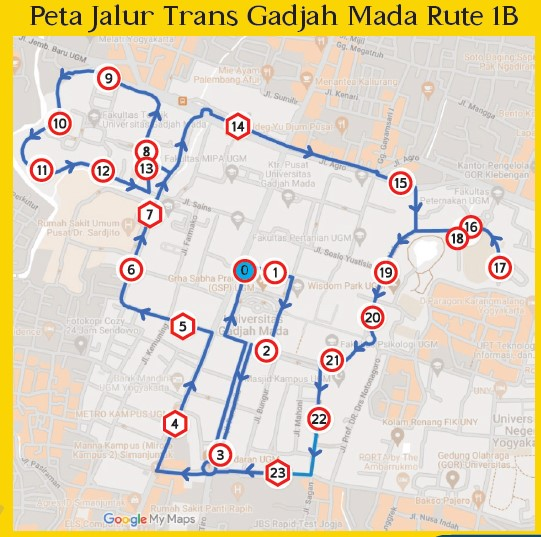
\includegraphics[width=6cm]{Peta-Jalur-Rute-1B.jpg}
	\caption{Rute 1B bus Trans Gadjah Mada}
	\label{Fig: tgm-1b}
\end{figure}

\section{Metode Penelitian}
Penelitian ini dilakukan pada tahun 2023 menggunakan modul GNSS Teseo-LIV3FL dan \textit{development board} STM32 Nucleo-WL55JC1. Lokasi penelitian berada di lingkungan Universitas Gadjah Mada dan sekitarnya. Adapun konfigurasi konstelasi yang digunakan adalah GPS, BeiDou, Galileo, dan QZSS. Pada penelitian ini akan dilakukan tiga pengujian. Pengujian \textit{rapid static survey} dan mode daya rendah hanya meninjau modul GNSS-nya saja, sedangkan pengujian lainnya akan menguji sistem secara keseluruhan.

\begin{table}[htb!]
	\caption{Lokasi Pengujian \textit{Rapid Static Survey}}
	\centering
	\renewcommand{\arraystretch}{1.5}
	\begin{tabular}{cc}
		\hline
		\textbf{Skenario} & \textbf{Lokasi} \\\hline
		\textit{Basement} &Ruang Bawah Tanah Fisipol UGM\\
		Dalam Ruangan & Lantai 5 SGLC Fakultas Teknik UGM\\
		Ruangan Semi Terbuka &  Selasar Grha Sabha Pramana\\
		Ruang Terbuka & Lapangan Pancasila\\
		\hline
	\end{tabular}
	\label{tab: 3-rss-location}
\end{table}

\textit{Rapid Static Survey} dilakukan untuk meninjau performa modul GNSS dalam keadaan diam. Pengujian dilakukan dengan meletakan modul di satu tempat dan merekam data selama satu jam. Untuk menerima kalimat NMEA dari modul, digunakan perangkat USB \textit{to} TTL dengan konfigurasi \textit{baud rate} 9600 bps. Pengujian ini dilakukan dalam empat buah skenario, yaitu \textit{basement}, dalam ruangan, ruang semi terbuka, dan ruang terbuka. Lokasi setiap skenario \textit{Rapid Static Survey} ditunjukan oleh Tabel \ref{tab: 3-rss-location}.

Salah satu fitur unggulan dari modul GNSS Teseo-LIV3FL adalah memiliki mode daya rendah. Pengujian mode daya rendah akan meninjau arus yang mengalir pada modul ketika mode daya rendah diaktifkan. Algoritma mode daya rendah yang digunakan adalah algoritma periodik.

Setelah meninjau performa \textit{multi-constellation} pada modul GNSS, langkah selanjutnya adalah menguji sisetm secara keseluruhan di Bus Trans Gadjah Mada. Pada penelitian ini, rute yang dipilih adalah Rute 1B (Gambar \ref{Fig: tgm-1b}). Waktu tempuh pengujian ini kurang lebih adalah selama satu jam yang diawali pada halte ke-14 dan diakhiri pada halte yang sama.

\section{Hasil Pengujian}
\subsection{\textit{Rapid Static Survey}}
\begin{table*}[tbp]
	\centering
	\renewcommand{\arraystretch}{1.5}
	\caption{Rata-Rata Hasil Pengamatan \textit{Rapid Static Survey}}
	\label{tab: 4-rss-summary}
	\begin{tabular}{ccccccc}
		\hline
		\textbf{Skenario} & \textbf{HDOP} & \textbf{VDOP} & \textbf{PDOP} & \textbf{Visibilitas Satelit} & \textbf{CEP} & \textbf{MAD} \\
		&  & &  & (buah) & (m) & (m) \\
		\hline
		1 & 6,67 & 8,27 & 10,67 & 7,60 & 32,69 & 24,11 \\
		2 & 2,79 & 2,48 & 8,40 & 10,93 & 12,14 & 8,46 \\
		3 & 0,91 & 1,49 & 1,75 & 14,32 & 13,83 & 3,06 \\
		4 & 0,65 & 1,12 & 1,30 & 21,14 & 6,12 & 1,21 \\
		\hline
	\end{tabular}
\end{table*}

Pengujian \textit{rapid static survey} dilakukan dengan cara menaruh modul GNSS di satu titik selama 15 menit s.d. 2 jam. Setiap skenario pengujian dibedakan berdasarkan penghalang di sekitarnya. Pada penelitian ini, durasi dari pengujian di setiap skenario adalah selama 1 jam. Parameter yang diamati dalam pengujian ini adalah HDOP, VDOP, PDOP, visibilitas satelit, \textit{Circular Error Probability} (CEP), dan \textit{Mean Average Deviation} (MAD). Hasil pengujian setiap skenario ditunjukan oleh Tabel \ref{tab: 4-rss-summary}.

\begin{table}[h]
	\caption{Rentang Nilai DOP}
	\centering
	\renewcommand{\arraystretch}{1.5}
	\begin{tabular}{cc}
		\hline
		\textbf{DOP} & \textbf{Klasifikasi}\\
		\hline 
		$<$1 & Ideal\\
		1 - 2 & Sangat Baik\\
		2 - 5 & Cukup \\ 
		5 - 10 & Sedang\\
		10 - 20 & Buruk\\ 
		$>$20 & Sangat Buruk\\
		\hline
	\end{tabular}
	\label{tab: 3-dop-class}
\end{table}

Skenario 1 dilakukan di \textit{basement} milik Fakultas Ilmu Sosial dan Politik UGM. Keadaan sekitar pengujian ditutupi oleh konstruksi beton dengan sedikit daerah terbuka yang memungkinkan sinar matahari untuk masuk. Keadaan tersebut tentunya akan sulit untuk ditembus oleh isyarat GNSS. Meskipun terhalang dengan beton, tetapi modul GNSS Teseo-LIV3FL dapat menerima isyarat GNSS dengan cukup baik ditunjukan oleh visibilitas satelit rata-rata sebanyak 7,60 buah. Rata-rata HDOP, VDOP, dan PDOP yang didapat adalah 6,67; 8,27; dan 10,67. Berdasarkan Tabel \ref{tab: 3-dop-class}, rata-rata nilai HDOP dan VDOP yang didapat berada dalam rentang sedang, sedangkan PDOP-nya berada dalam rentang sangat buruk. Selain itu, ketelitian hasil pengukuran modul Teseo-LIV3FL menurut nilai MAD dan CEP adalah sebesar 24,11 meter dan 32,69 meter.

Selanjutnya, Skenario 2 dilakukan di Lantai 5 SGLC Fakultas Teknik. Pemilihan lokasi tersebut ditujukan untuk menguji modul Teseo-LIV3FL di lingkungan yang sedikit lebih terbuka. Hasil pengujian menunjukan terjadi peningkatan performa pada modul Teseo-LIV3FL. Dapat dilihat bahwa rata-rata visibilitas satelit meningkat menjadi 10,92. Selain itu, rata-rata nilai HDOP dan VDOP sudah berada dalam standar minimum sedangkan PDOP-nya masih berada dalam kategori cukup. Tingkat kepresisian modul juga mengalami peningkatan seperti ditunjukan dengan nilai rata-rata CEP sebesar 12,13 meter dan MAD sebesar 8,46 meter.

Skenario 3 dilakukan di selasar Grha Sabha Pramana Universitas Gadjah Mada. Pengujian skenario ini dilakukan untuk meninjau performa modul GNSS di ruang semi-terbuka. Pada skenario ini, performa modul Teseo-LIV3FL menjadi lebih baik yang ditunjukan oleh penurunan nilai ketiga DOP. Nilai HDOP sudah termasuk dalam klasifikasi ideal, sedangkan VDOP dan HDOP berada dalam klasifikasi sangat baik. Selain itu, rata-rata visibilitas satelit meningkat menjadi 14,32. Pada pengujian ini terjadi sedikit peningkatan pada nilai CEP menjadi 13,83 meter, tetapi nilai MAD-nya menurun menjadi 6,12 meter.

 Terakhir, Skenario 4 dilakukan di Lapangan Pancasila Universitas Gadjah Mada. Lapangan pancasila dipilih karena merepresentasikan kondisi ideal penempatan modul GNSS, yaitu ruang terbuka tanpa halangan. Hasil pengujian skenario ini merupakan hasil paling baik dari tiga skenario sebelumnya dengan rata-rata visibilitas satelit 21,14. Nilai HDOP, VDOP, dan PDOP masih dalam rentang yang sama, tetapi sedikit lebih baik. Rata-rata nilai CEP dari pengujian ini adalah 6,12 meter  dan nilai MAD sebesar 1,21 meter. Meskipun nilai CEP yang didapat tidak sama dengan \textit{datasheet}, tetapi nilai tersebut sudah cukup baik untuk aplikasi pelacak kendaraan.

\begin{figure}[htb!]
	\centering
	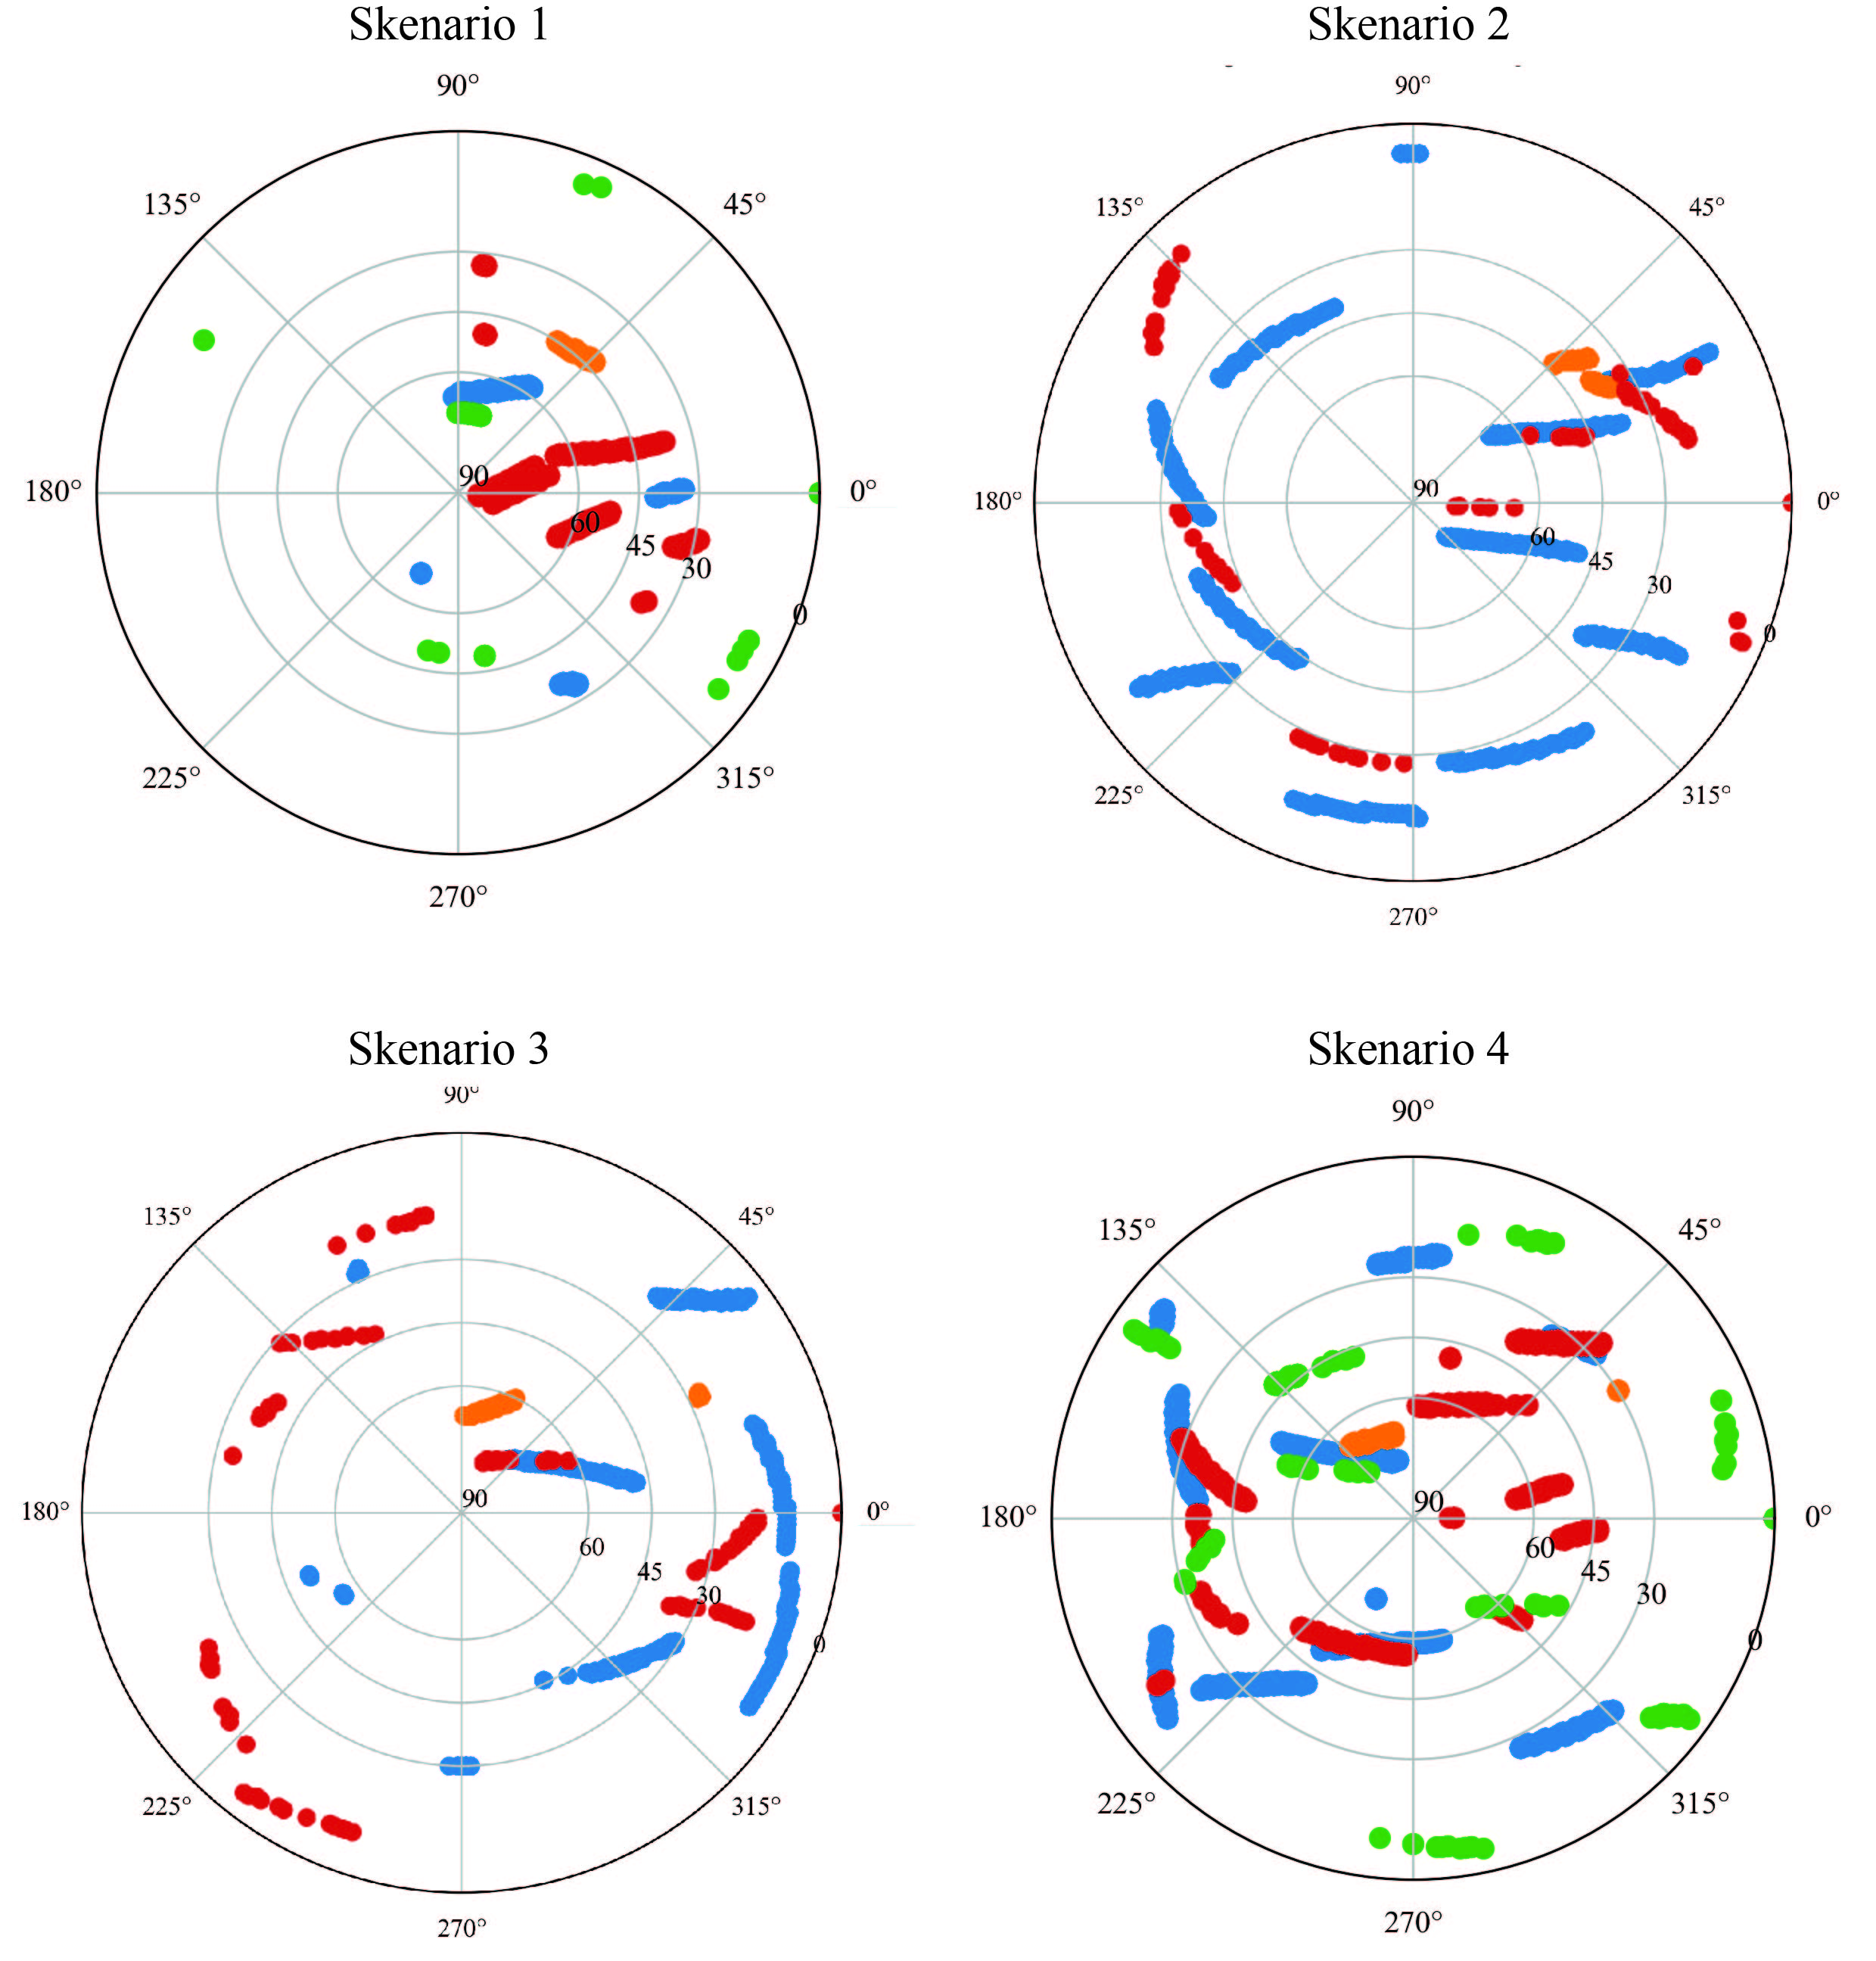
\includegraphics[width=8cm]{skyplot.jpg}
	\caption{\textit{Sky plot} Hasil \textit{rapid static survey} (biru: GPS; merah: BeiDou; hijau: Galileo; dan oranye: QZSS)}
	\label{fig: 4-skyplot}
\end{figure}

Tren nilai PDOP cenderung menurun untuk setiap skenario. Nilai PDOP dipengaruhi oleh geometri dari satelit. Sebagai contoh, nilai PDOP pada skenario 1 sangatlah tinggi dan persebaran satelitnya hanya mengisi $\frac{1}{4}$ bagian lingkaran seperti ditunjukan oleh Gambar \ref{fig: 4-skyplot}. Di sisi lain, \textit{sky plot} pada skenario 4 menunjukan bahwa satelitnya lebih tersebar di langit karena memenuhi seluruh lingkaran. Hal tersebut sejalan dengan nilai PDOP-nya yang menurun.

\subsection{Algoritma Mode Daya Rendah}
Modul Teseo-LIV3FL memiliki fitur yang memungkinkan modul untuk bekerja dalam mode serendah mungkin. Algoritma mode daya rendah yang digunakan bekerja secara periodik. Setelah mendapat fiksasi, modul akan menuju mode \textit{standby} selama periode waktu tertentu. Hal yang sama juga terjadi jika modul tidak mendapatkan fiksasi dalam periode waktu tertentu. 

\begin{figure}[htb!]
	\centering
	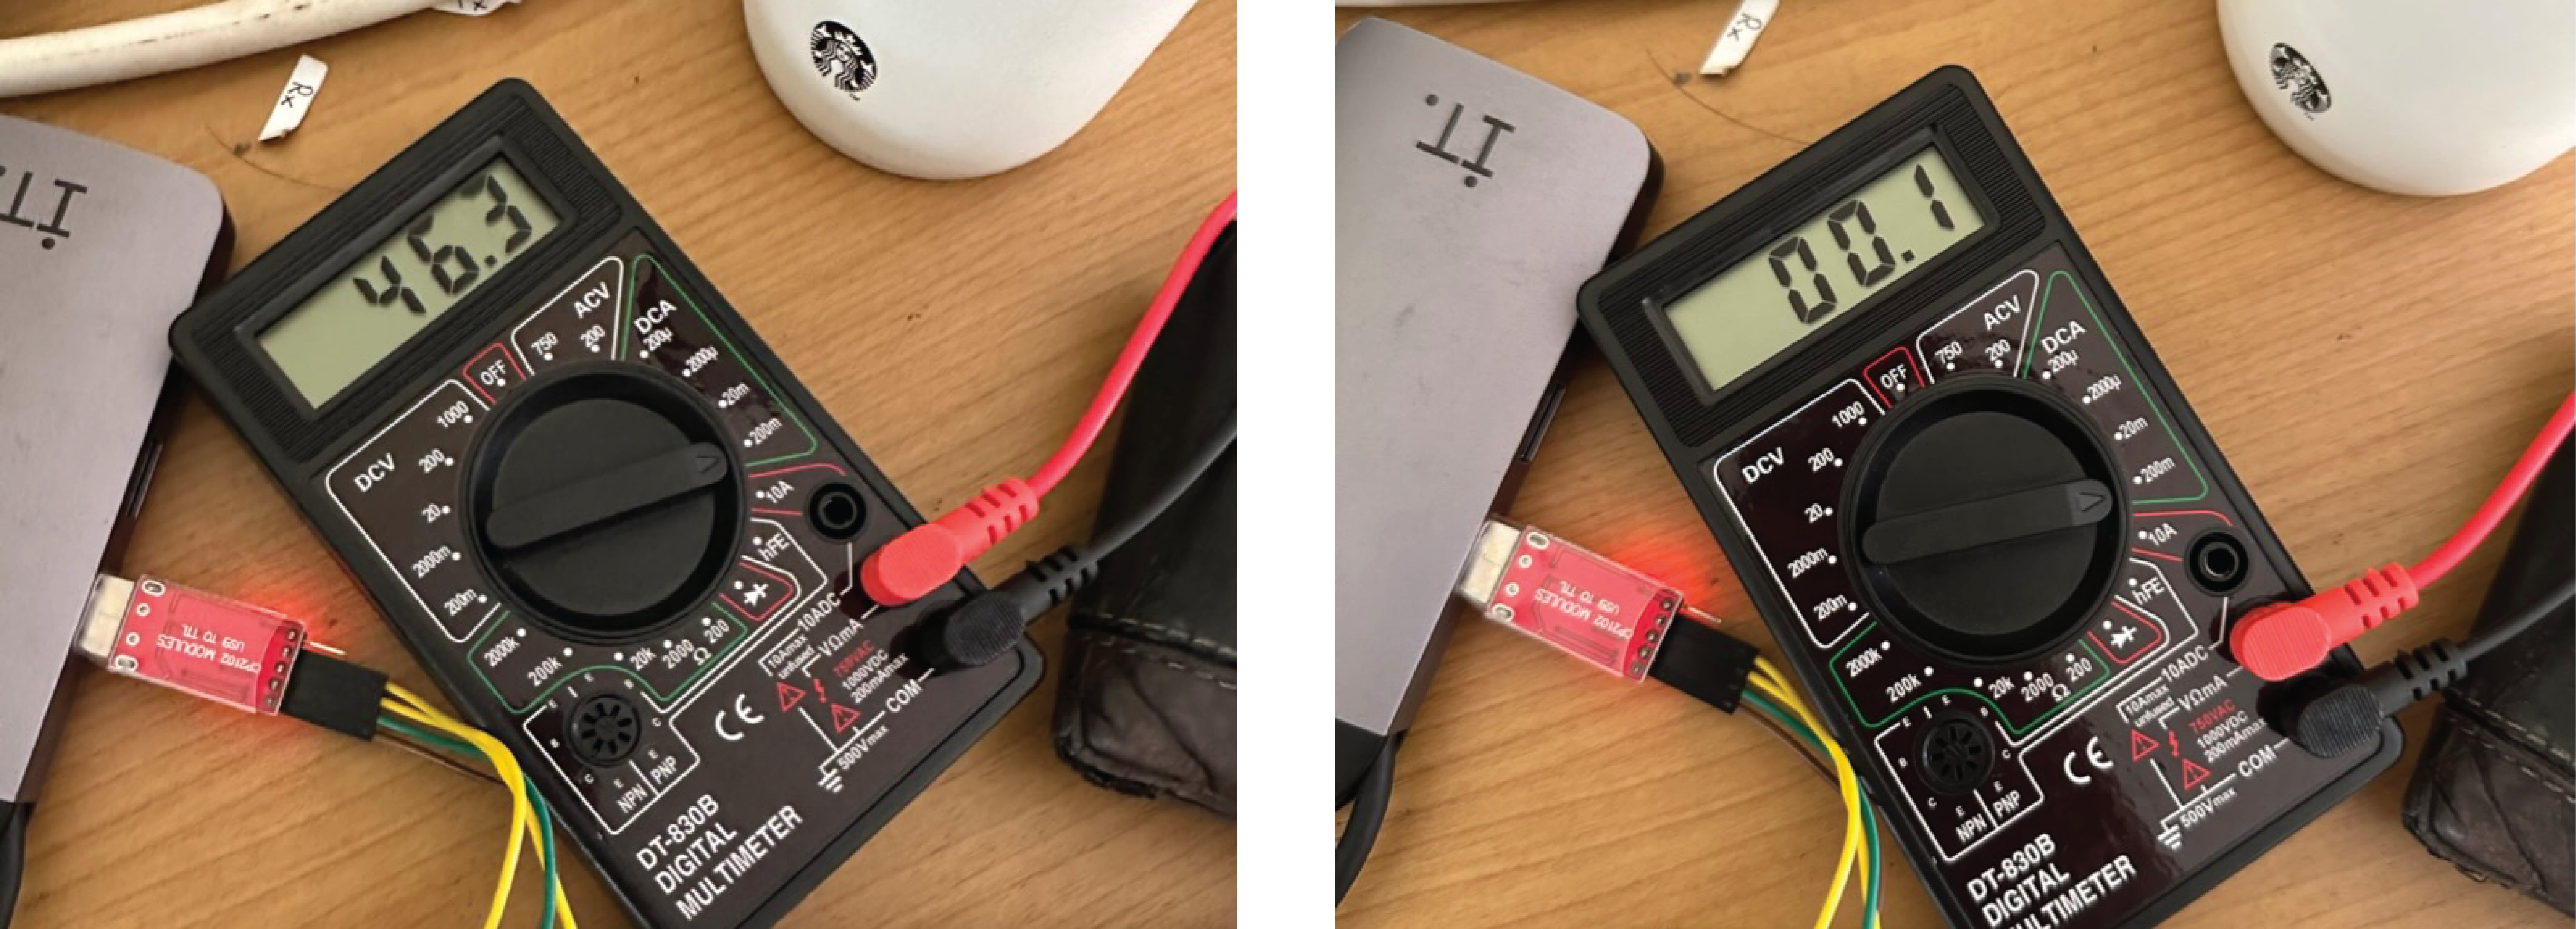
\includegraphics[width=8.7cm]{low-power-result.jpg}
	\caption{Pembacaan multimeter pada mode akuisisi (kiri) dan mode \textit{standby} (kanan)}
	\label{Fig: 4-low-power-result}
\end{figure}

Berdasarkan pengujian yang dilakukan, modul arus yang mengalir pada modul Teseo-LIV3FL pada mode \textit{standby} adalah sebesar 15 $\mu$A (Gambar \ref{Fig: 4-low-power-result} kanan) dan 65 mA (Gambar \ref{Fig: 4-low-power-result} kiri) pada mode akuisisi. Nilai yang didapat sudah mendekati \textit{datasheet}, yaitu 10 $\mu$A pada mode \textit{standby}. Selain meninjau arus yang mengalir pada modul, perlu ditinjau juga hasil pengukuran dari modul Teseo-LIV3FL.

\begin{table}[h]
	\centering
	\renewcommand{\arraystretch}{1.5}
	\caption{Performa Modul GNSS dengan Variasi Waktu \textit{Standby}}
	\label{tab: 4-lpm-var}
	\begin{tabular}{ccccc}
		\hline
		\textbf{Waktu \textit{Standby}} &\textbf{TTFF (s)} & \textbf{HDOP} & \textbf{Visibilitas Satelit} & \textbf{Fiksasi}\\
		\hline 
		1 menit & 8,47 & 1,5 & 9 & 3D\\
		2 menit & 11,24 & 1,1 & 8 & 3D\\
		3 menit & 11,47 & 1,8 & 8 & 3D\\
		4 menit & 19,46 & 2,6 & 5 & 2D\\
		5 menit & 20,65 & 3,5 & 5 & 2D\\
		6 menit & $\infty$ & - & - & -\\
		\hline
	\end{tabular}
\end{table}

Hasil pengujian dengan berbagai skenario waktu \textit{standby} ditunjukan pada Tabel \ref{tab: 4-lpm-var}. Jika waktu \textit{standby} diatur dalam rentang 1 hingga 3 menit, modul masih mendapat fiksasi 3D dengan sedikit perubahan pada parameter lainnya. Pada skenario 4 dan 5 menit, nilai \textit{time to first fix} (TTFF) menjadi lebih lama hingga 20 detik. Selain itu, modul hanya mendapat fiksasi 2D saja. Jika waktu \textit{standby} diatur menjadi lebih dari 5 menit, modul tidak mendapat fiksasi sama sekali.

Hal tersebut diakibatkan ketika modul GNSS dalam keadaan \textit{standby} yang cukup lama, data efemeris yang lama menjadi usang dan modul perlu mengunduh data efemeris yang baru. Selain itu, modul GNSS juga bekerja dengan prinsip \textit{line-of-sight}. Tentunya keadaan \textit{line-of-sight} setelah modul GNSS kembali ke mode akuisisi telah berbeda dengan \textit{line-of-sight} modul tepat sebelum masuk ke mode \textit{standby}.

\begin{figure}[htb!]
	\centering
	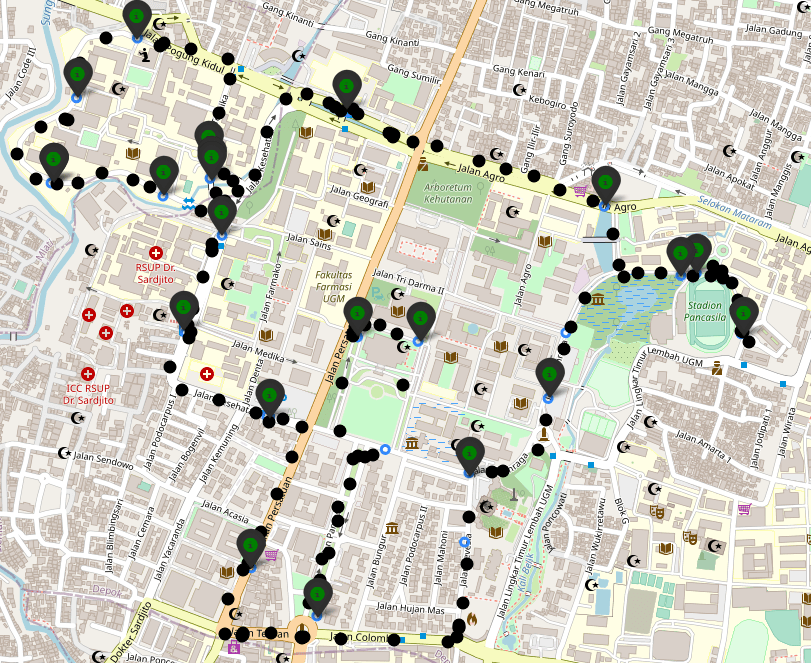
\includegraphics[width=7cm]{tracked-route.png}
	\caption{Hasil pelacakan sistem di bus Trans Gadjah Mada rute 1B}
	\label{Fig: 4-tgm-tracked}
\end{figure}

\subsection{Pengujian pada Bus Trans Gadjah Mada}
\begin{table}[H]
	\caption{Rangkuman performa hasil pengujian di bus Trans Gadjah Mada rute 1B}
	\centering
	\renewcommand{\arraystretch}{1.5}
	\begin{tabular}{cc}
		\hline
		\textbf{Parameter} & \textbf{Rata-Rata} \\\hline
		HDOP & 1,12\\
		VDOP & 1,72\\
		PDOP &  1,98\\
		Visibilitas Satelit & 9,98\\
		\hline
	\end{tabular}
	\label{tab: 4-tgm-performance}
\end{table}

Pengujian di Bus Trans Gadjah Mada dilakukan untuk meninjau performa sistem jika dalam keadaan bergerak. Durasi pengujian adalah selama satu jam yang diawali di Halte 0 hingga kembali ke Halte 0. Hasil pelacakan posisi ditunjukan oleh Gambar \ref{Fig: 4-tgm-tracked}. Dapat dilihat juga bahwa hasil pelacakan bus sudah mendekati rute pada Gambar \ref{Fig: tgm-1b}. Titik berwarna hitam menunjukan posisi saat ini, sedangkan titik berwarna hijau menunjukan posisi bus ketika sistem mendeteksi bus sedang berhenti di satu halte tertentu. Rangkuman performa hasil pengujian di Trans Gadjah Mada Rute 1B ditunjukan oleh Tabel \ref{tab: 4-tgm-performance}.

\begin{figure}[htb!]
	\centering
	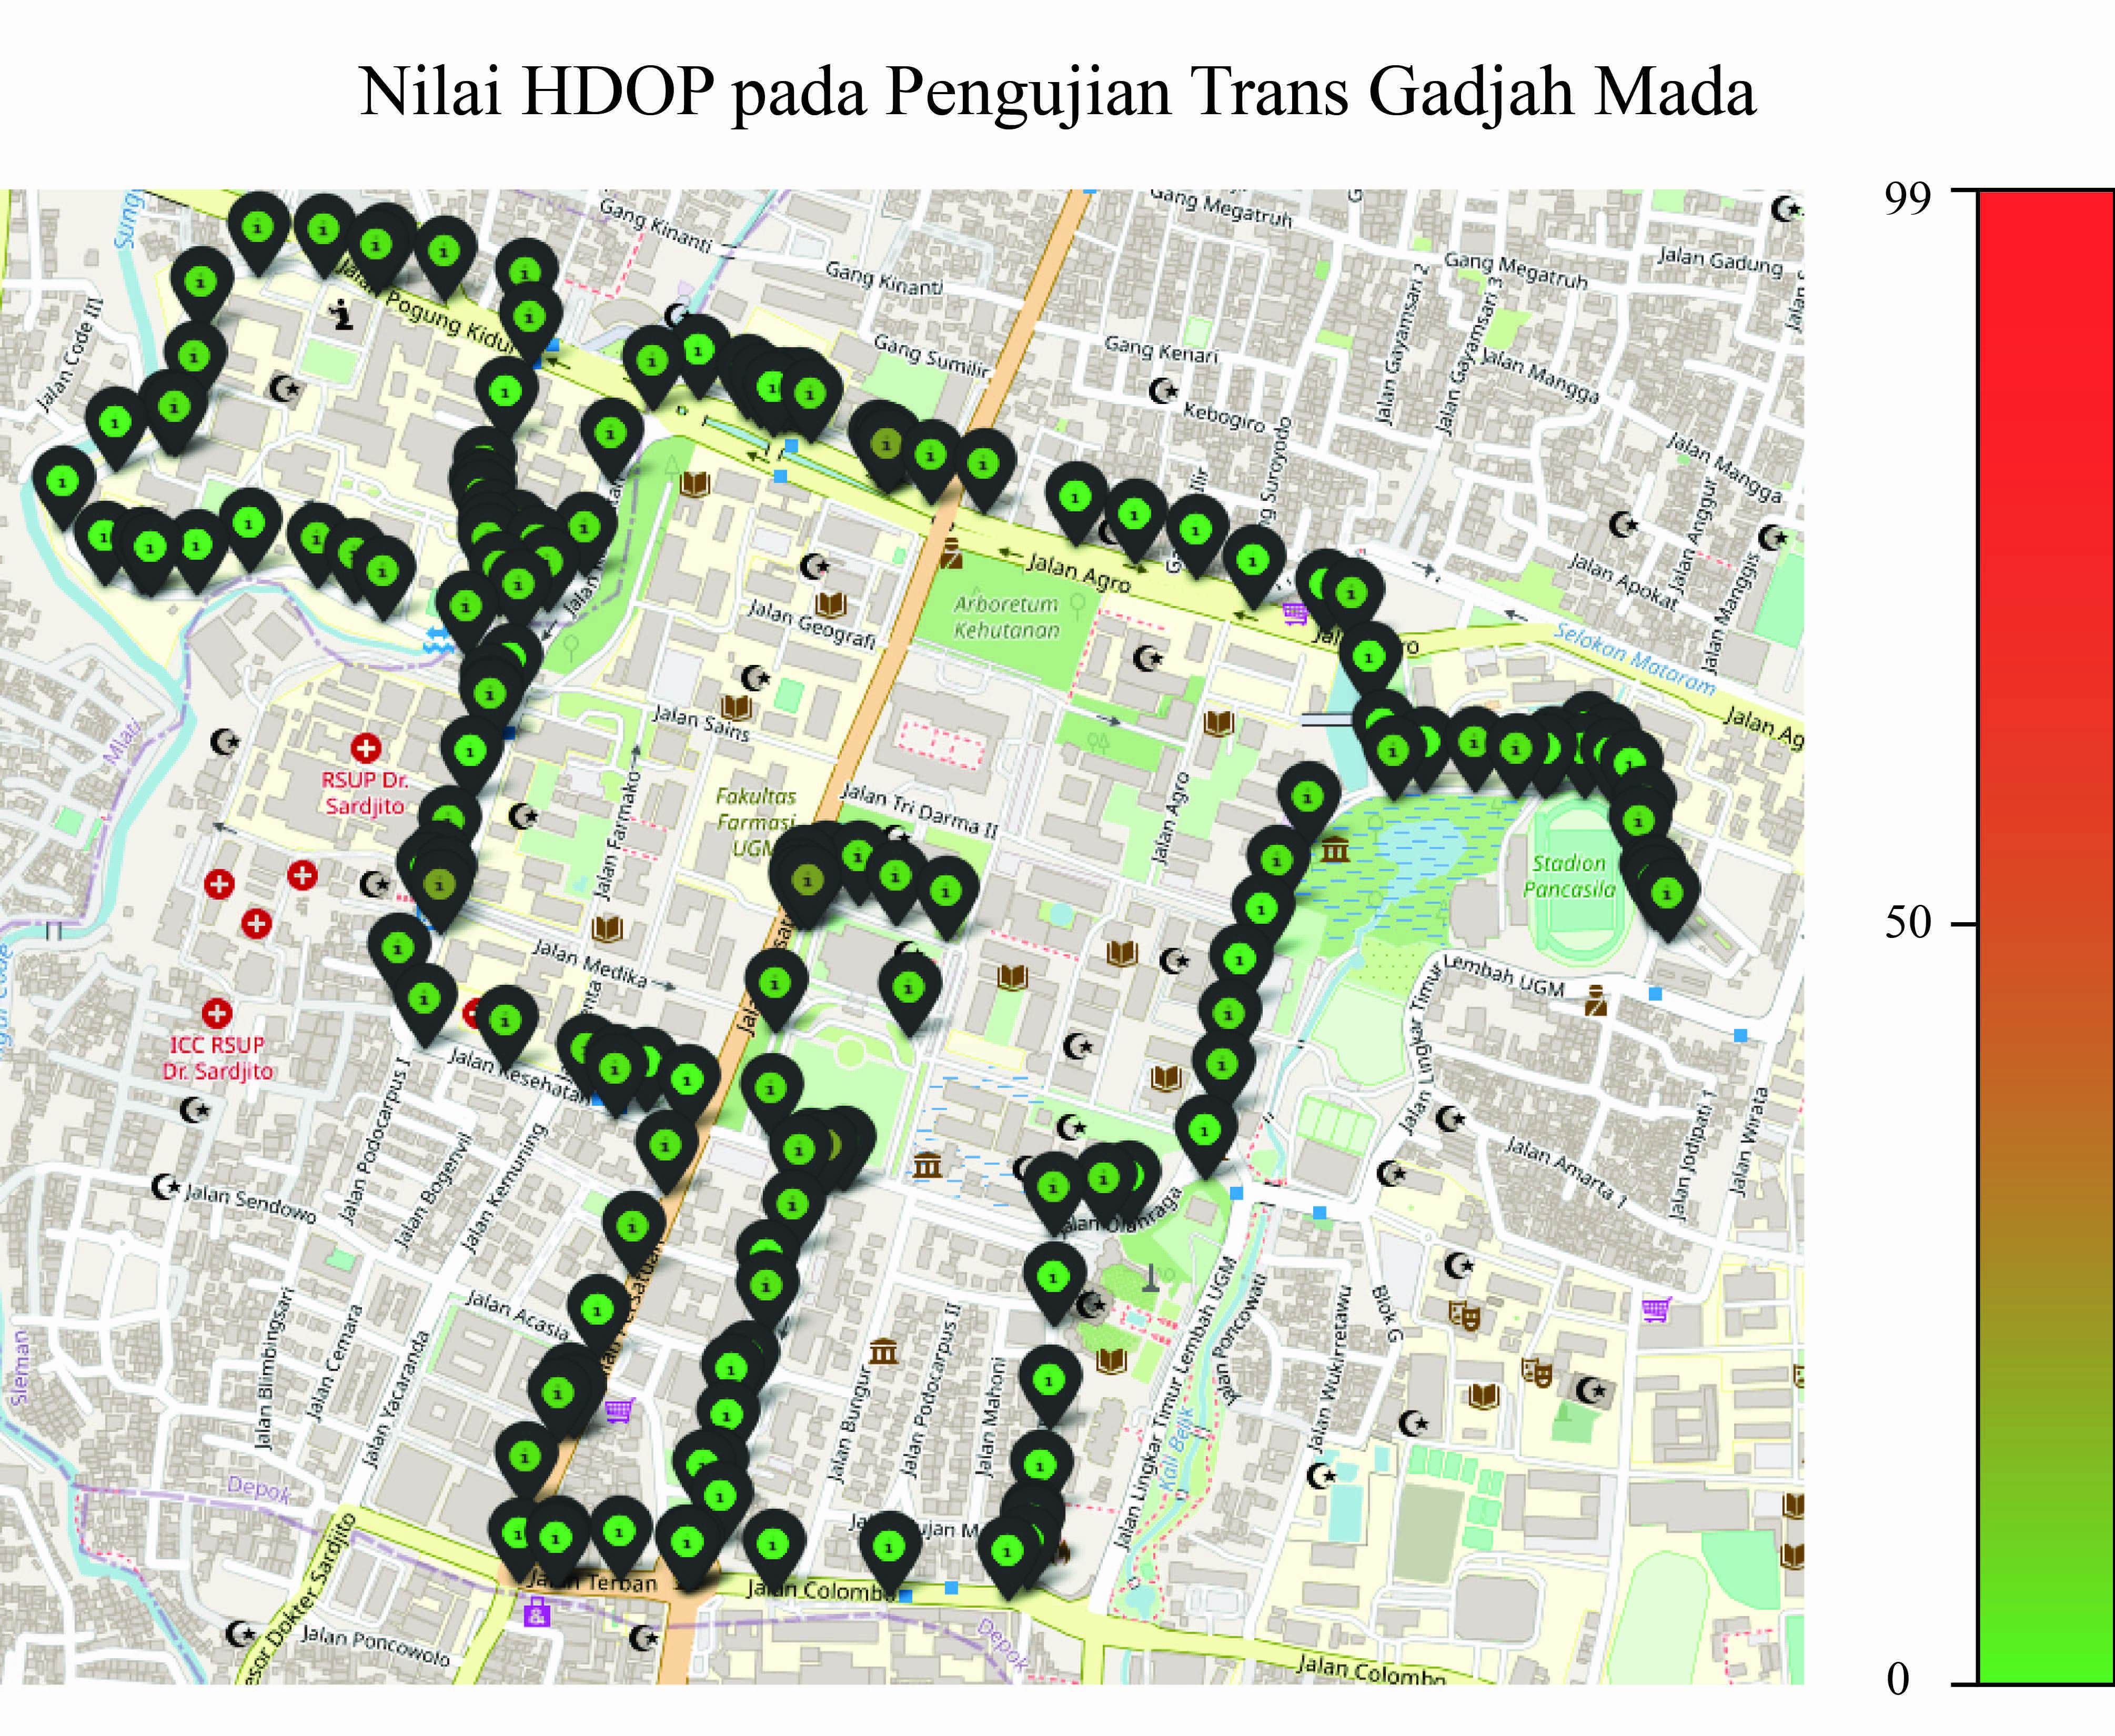
\includegraphics[width=7cm]{moving-HDOP.jpg}
	\caption{Nilai HDOP pengujian di bus Trans Gadjah Mada rute 1B}
	\label{Fig: 4-tgm-hdop}
\end{figure}

Kualitas hasil pelacakan pada pengujian ini dapat ditinjau dari nilai HDOP-nya. Pada penelitian ini hanya akan ditinjau dari nilai HDOP-nya saja karena pelacakan yang dilakukan hanya pada posisi di bidang horizontal saja. Rata-rata nilai HDOP pada pengujian ini adalah 1,12 atau sangat baik. Berdasarkan Gambar \ref{Fig: 4-tgm-hdop}, nilai HDOP di semua titik memiliki warna hijau atau berada dalam rentang ideal dan sangat baik. Hal tersebut menunjukkan bahwa tingkat akurasi pada bidang horizontalnya berada pada rentang yang baik dan layak untuk digunakan.

\begin{figure}[htb!]
	\centering
	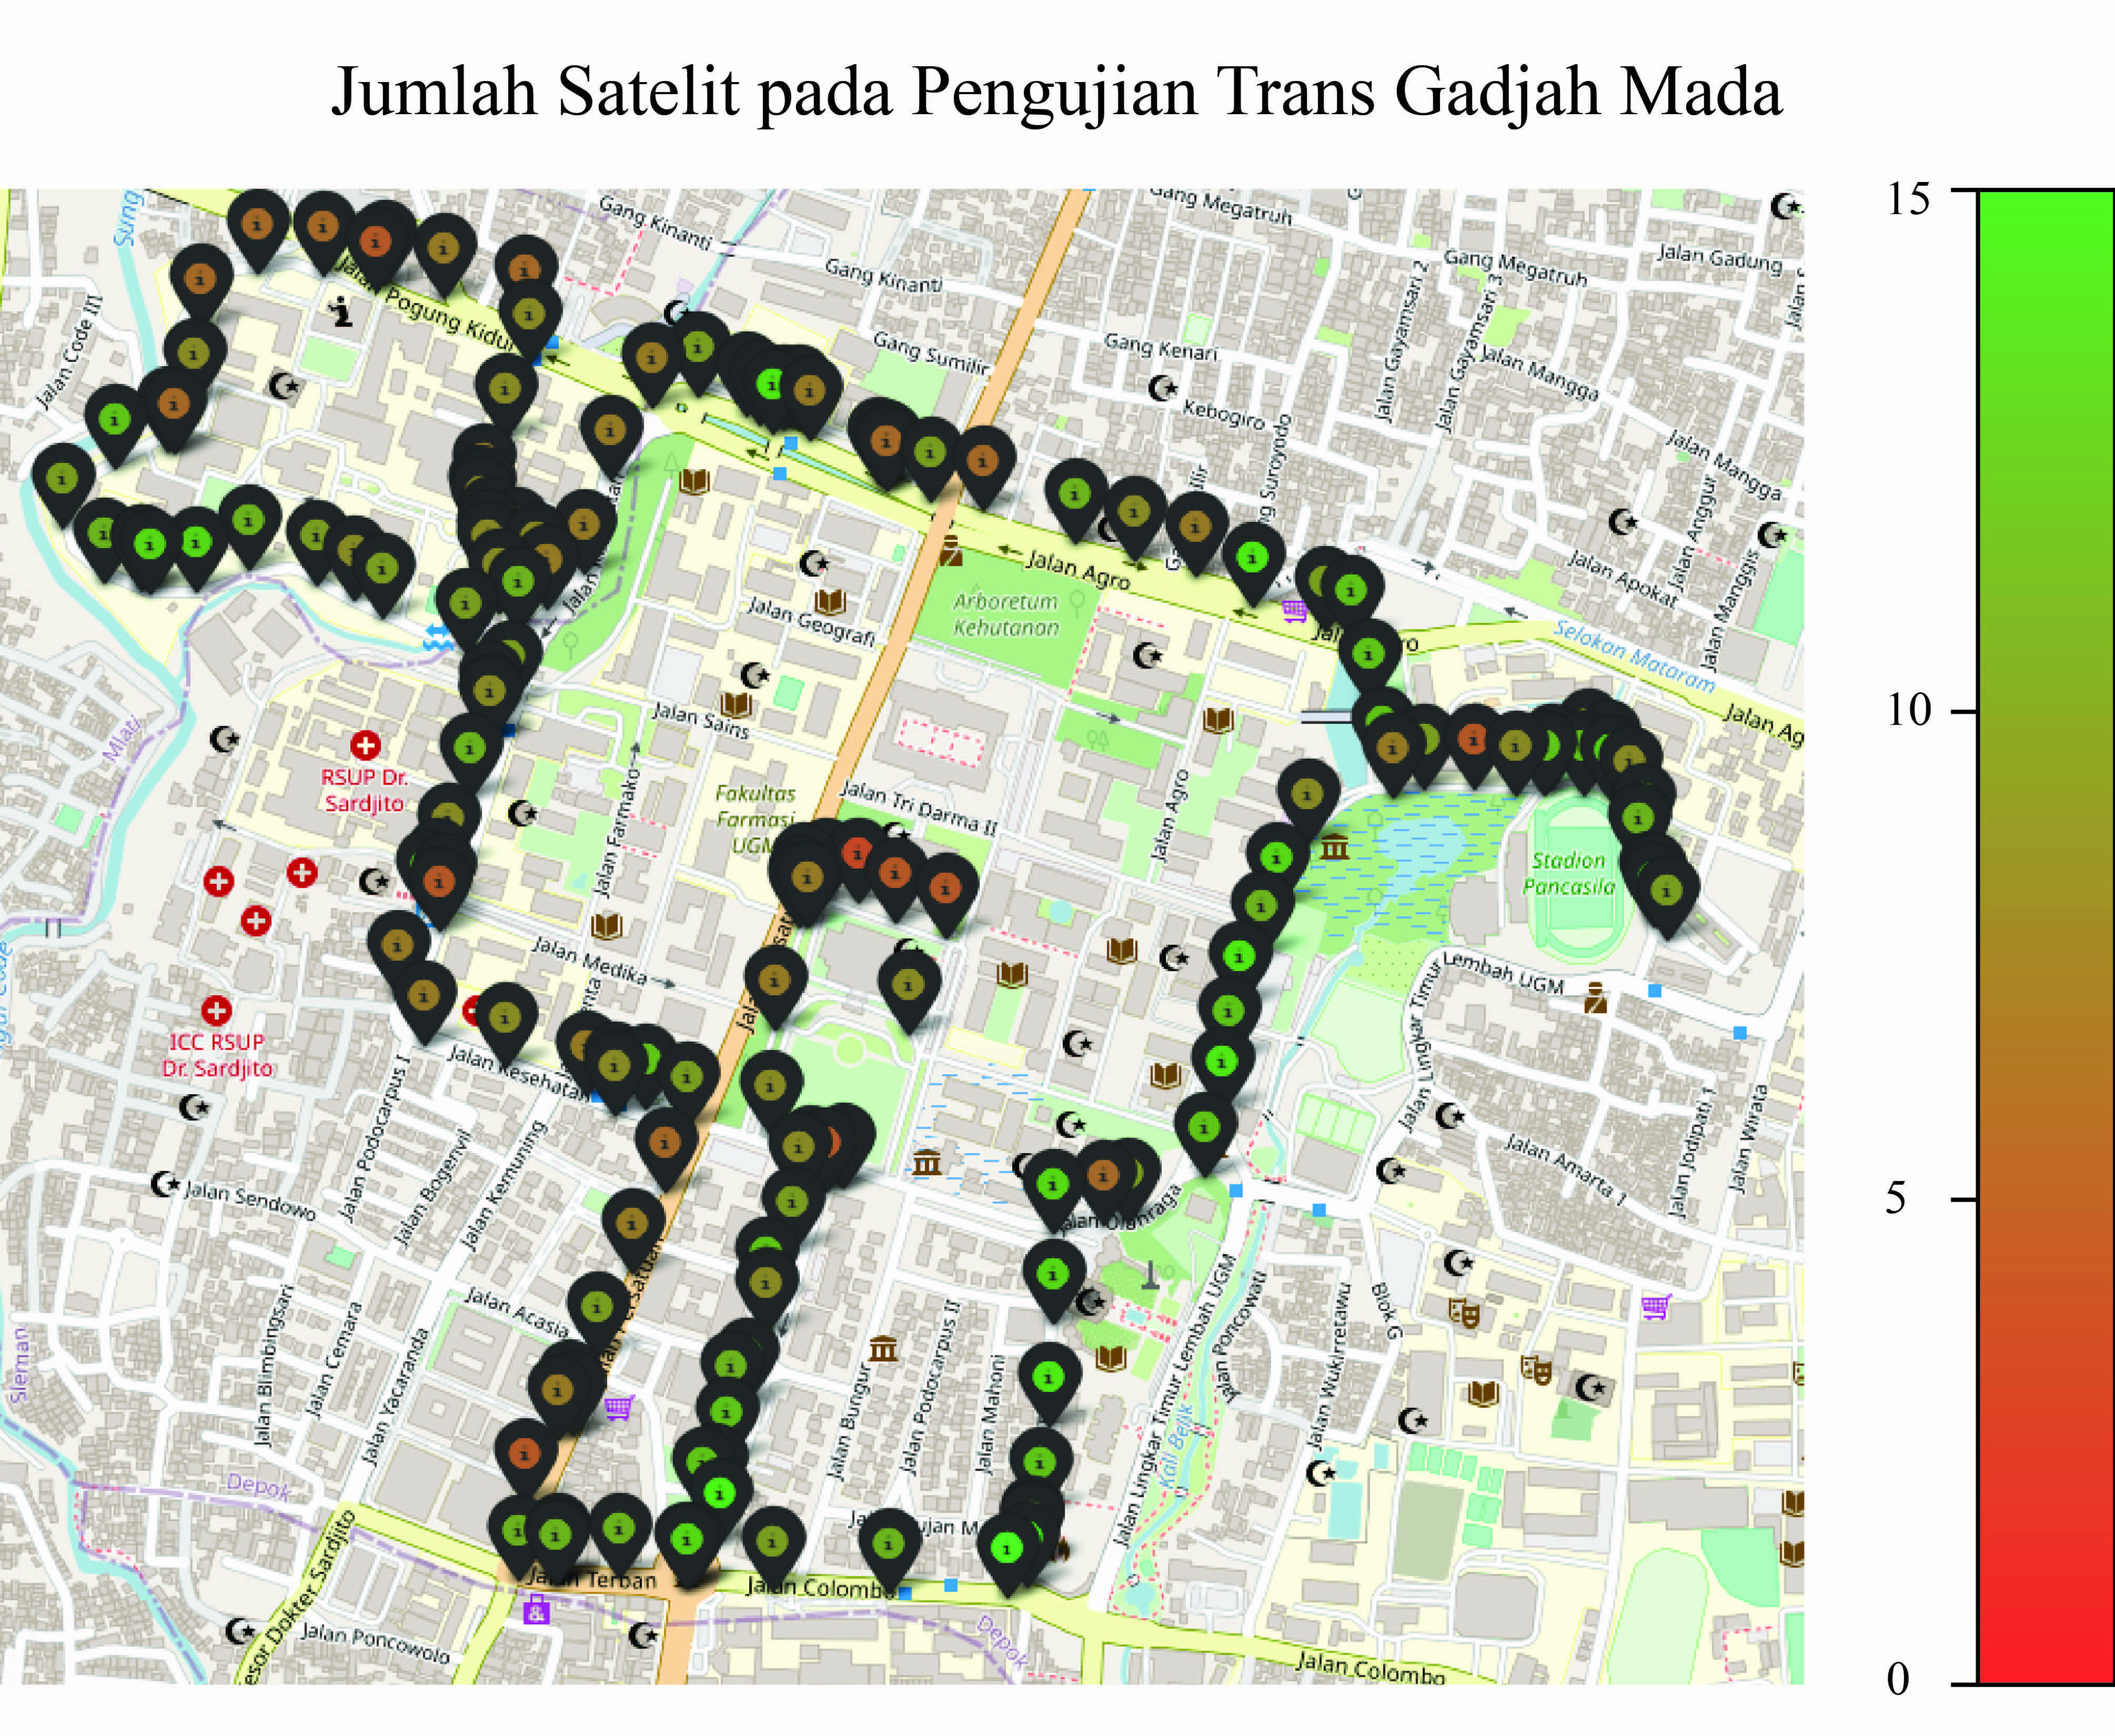
\includegraphics[width=7cm]{moving-SATS.jpg}
	\caption{Visibilitas satelit pengujian di bus Trans Gadjah Mada rute 1B}
	\label{Fig: 4-tgm-sats}
\end{figure}

Selain HDOP, visibilitas satelit juga berperan penting terhadap hasil pelacakan. Jika dilihat pada Gambar \ref{Fig: 4-tgm-sats}, tidak semua titik memiliki visibilitas satelit lebih dari 10 buah (titik berwarna hijau). Rata-rata visibilitas satelit pada pengujian ini adalah sebanyak 9,98 buah. Visibilitas satelit paling rendah pada pengujian ini adalah sebanyak 6 buah satelit. Salah satu titik dengan visibilitas satelit paling rendah adalah di sekitar halte Rumah Sakit Dr. Sardjito. Hal tersebut dapat diakibatkan oleh banyaknya gedung dan pepohonan yang dapat menghalangi isyarat GNSS. Meskipun terdapat beberapa titik dengan visibilitas satelit sejumlah enam buah, nilai HDOP pada lokasi tersebut tetap berwarna hijau tua atau baik. Hal tersebut dikarenakan visibilitas satelit yang dimiliki sudah melebihi batas minimal visibilitas satelit untuk mendapat fiksasi 3D, yaitu empat buah satelit.

\section{Kesimpulan}
Hasil pengujian \textit{rapid static survey} menunjukan untuk mendapatkan performa terbaik dari modul Teseo-LIV3FL maka modul harus diletakan di lingkungan terbuka dengan halangan seminimal mungkin. Selain itu, algoritma mode daya rendah pada modul memungkinkan modul untuk bekerja dengan daya yang lebih rendah. Perlu diingat bahwa waktu \textit{standby} ideal sebelum modul kesulitan untuk mendapat fiksasi adalah kurang dari 6 menit. Terakhir, hasil pengujian secara langsung di bus Trans Gadjah Mada Rute 1B sudah sangat baik dengan rata-rata visibilitas satelit sebanyak 9,98 buah dan nilai HDOP rata-rata sebesar 1,12.

\bibliography{references}{}
\bibliographystyle{IEEEtran}

\end{document}
